%=================================================================
\section{Introduction}
\label{sec-intro}
\begin{itemize}
   \item Use recipe ingredients to categorize the cuisine.
   Given the name of the condiment, predict the cuisine to which the dish belongs.
   \item In the dataset,including the recipe ID, the dish, and the list of ingredients for each recipe (variable length).The data is stored in JSON format. \\
   1.train.json- A training set that contains the recipe ID, dish type, and ingredient list\\
   2.test.json- A test set containing a recipe ID and a list of ingredients\\
   3.sample_submission.csv-Properly formatted sample submission document
\end{itemize} 
\section{Data Analysis} \label{sec-preliminaries}

First of all, our work can be divided into the following steps:\\
(1)   Data Import And Introduction
\begin{itemize}
  \item Import the JSON file with Pandas:We can get the data set of dish names, including 39774 training data and 9944 test samples.To see the distribution of our data set and the total variety of dishes, we printed out some of the data samples.
  \begin{center}
    \begin{minipage}{1\linewidth}
     \centering
      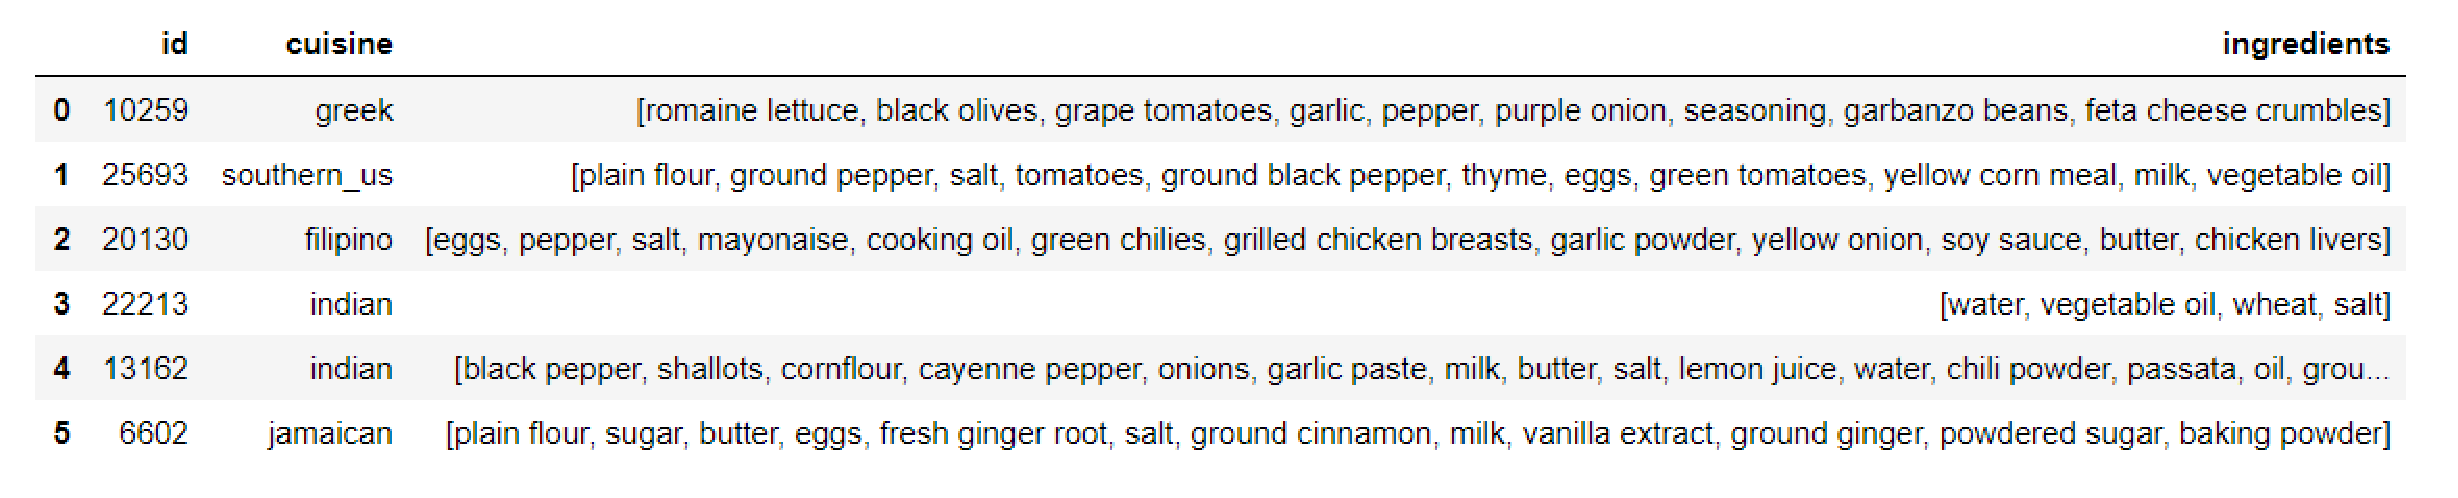
\includegraphics[width=0.6\textwidth]{pic01/a .eps}
    \end{minipage}
  
    \hfill
  \end{center}
  \item Total dish classification\\
        There are 20 dishes in total, which are:
        ['brazilian' 'british' 'cajun_creole' 'chinese' 'filipino' 'french'
         'greek' 'indian' 'irish' 'italian' 'jamaican' 'japanese' 'korean'
         'mexican' 'moroccan' 'russian' 'southern_us' 'spanish' 'thai'
         'vietnamese']
\end{itemize} 
(2)Analyze Data
\begin{itemize}
 \item The data set is divided into Features and Target Variables.
 \item Features:'ingredients', we were given the names of the ingredients contained in each dish;
Target variable:'cuisine', is the classification of cuisines that we want to predict.
 \item Extract the Feature of training data set into train_integredients variable
      Extract the Target Variables into the train_Targets variable.
\end{itemize} 
\begin{center}
  \begin{minipage}{1\linewidth}
  \centering
  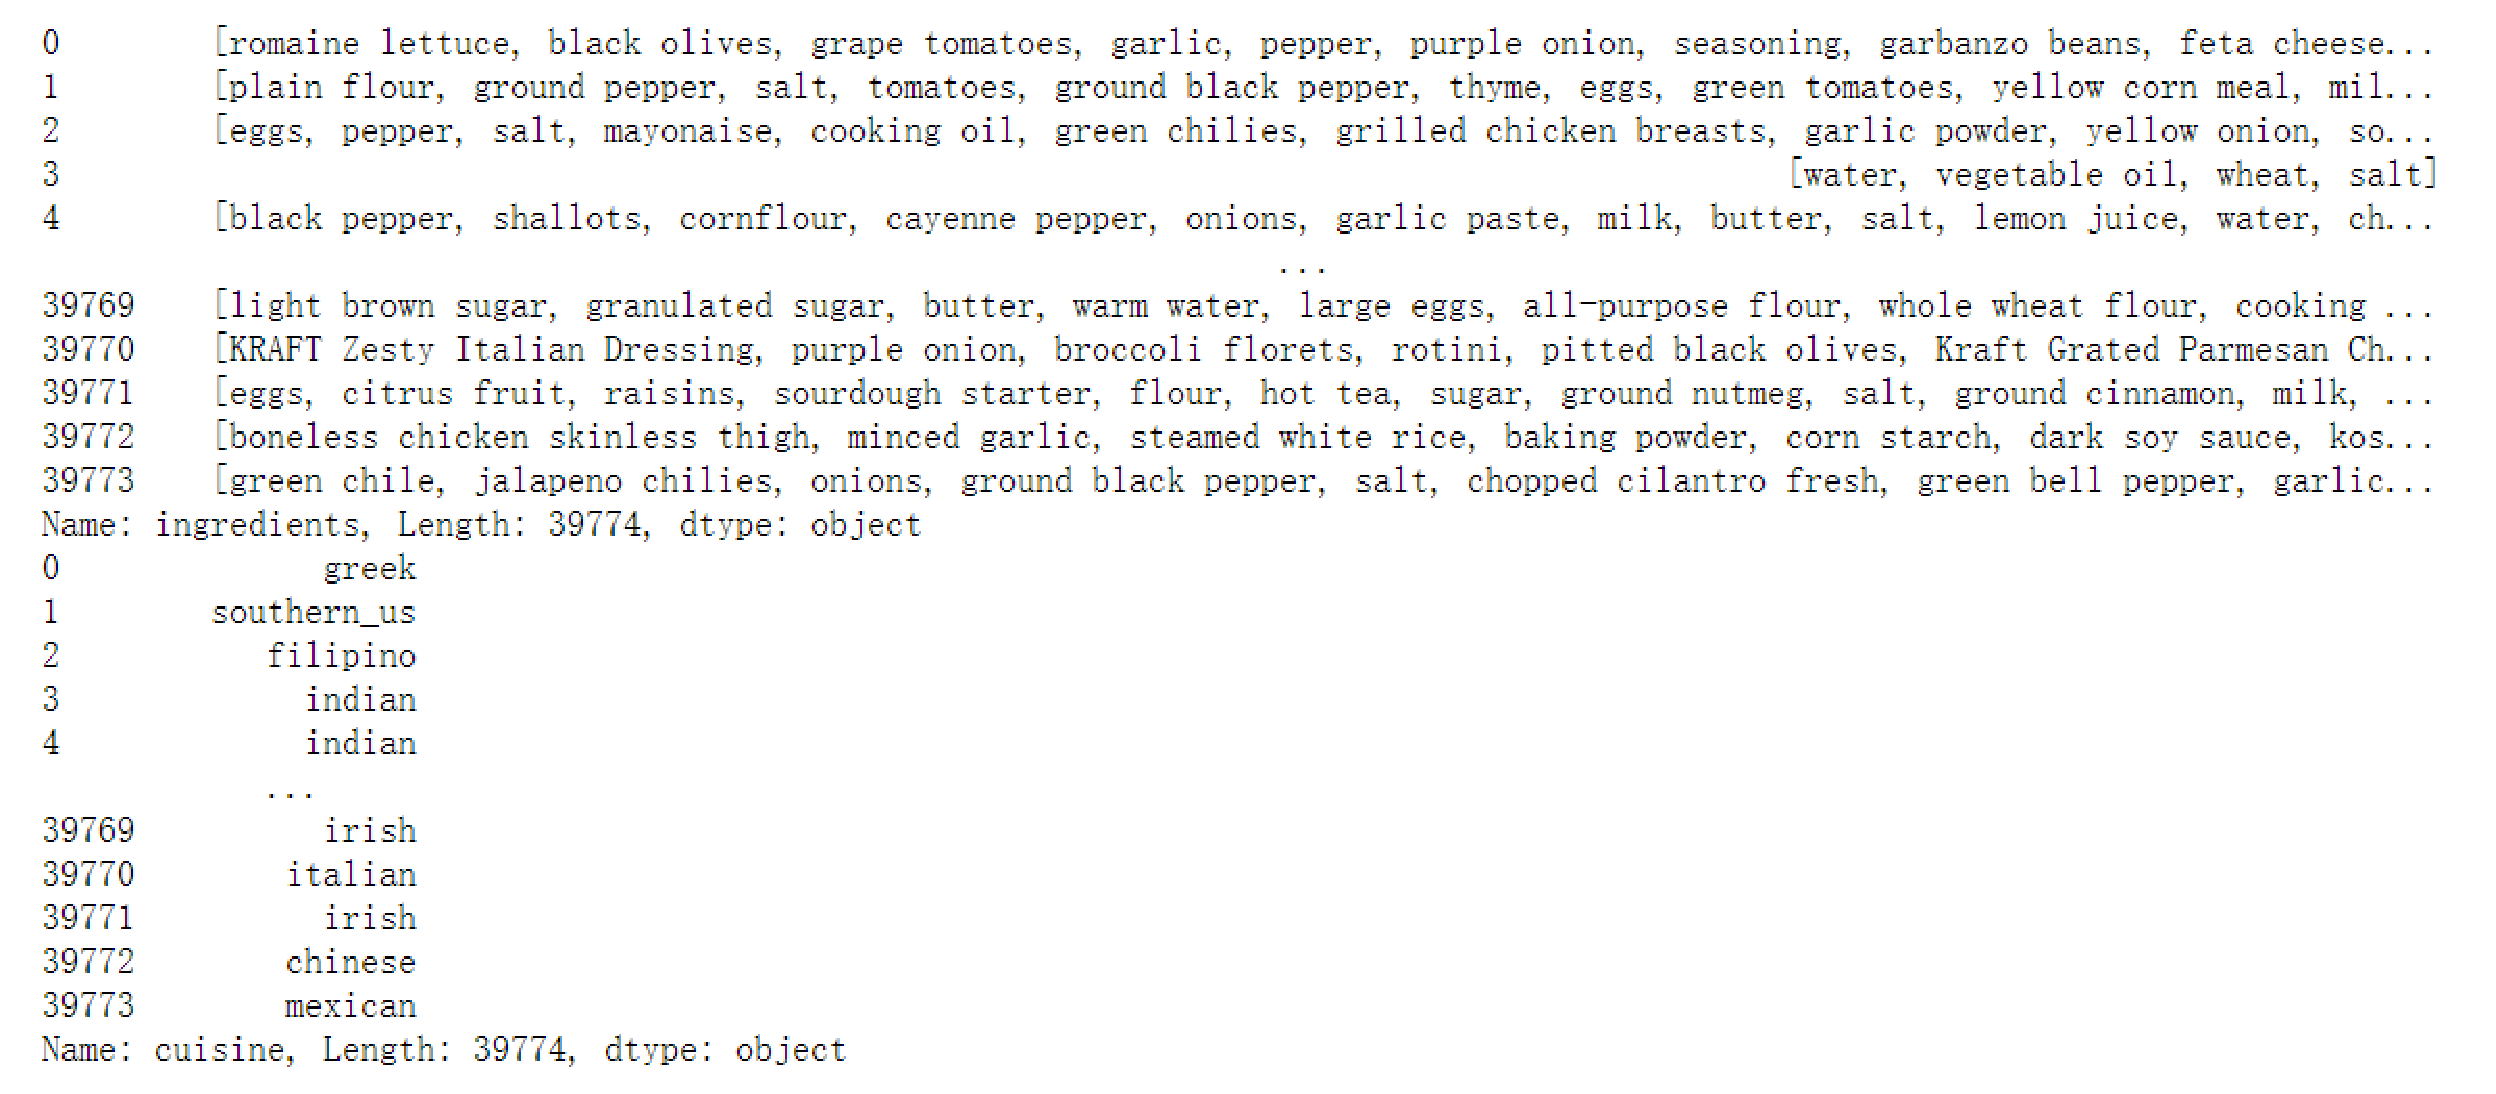
\includegraphics[width=0.7\textwidth]{pic01/b.eps}
\end{minipage}

  \hfill
\end{center}
(3) Data  Visualization\\What are the top 10 most frequently used ingredients?\\ What are the 10 most common ingredients in filipino,greek and Italian cuisine?
\begin{center}
  \begin{minipage}{0.5\linewidth}
    \centering
    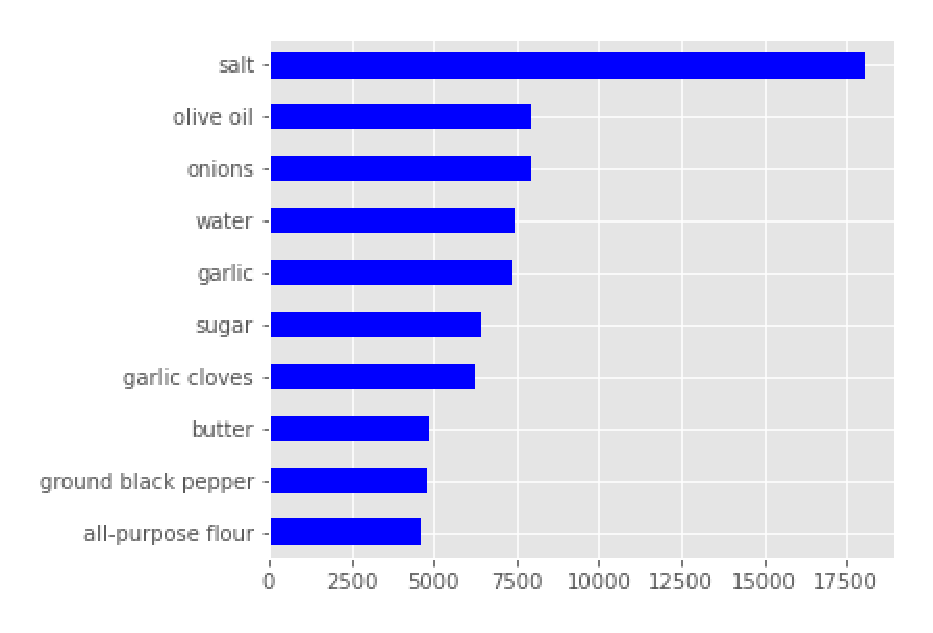
\includegraphics[width=0.5\textwidth]{pic01/cooking.eps}
  \end{minipage}
  
  \begin{minipage}{0.5\linewidth}
    \centering
    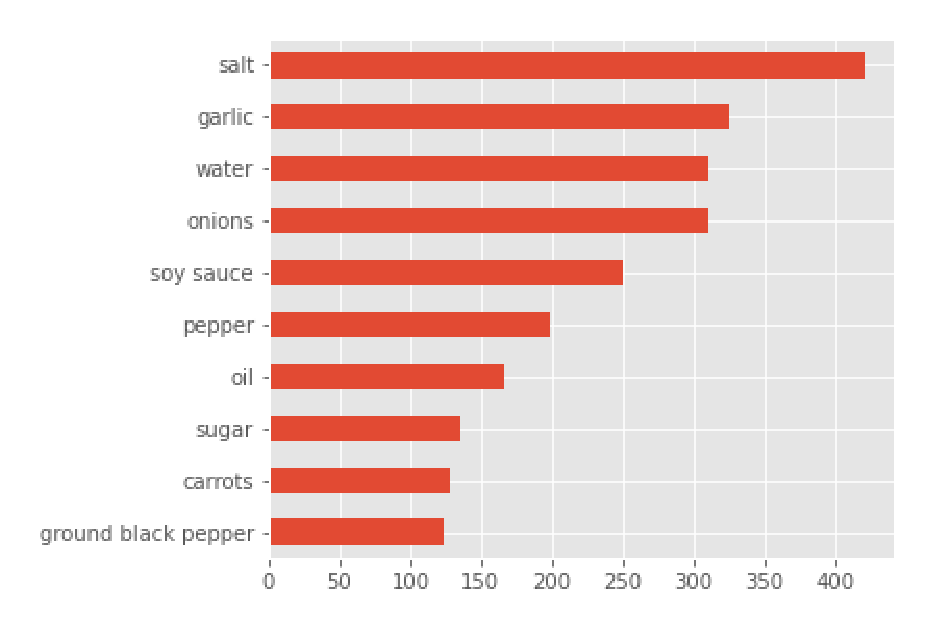
\includegraphics[width=0.5\textwidth]{pic01/filipino.eps}
  \end{minipage}
  
  \begin{minipage}{0.5\linewidth}
    \centering
      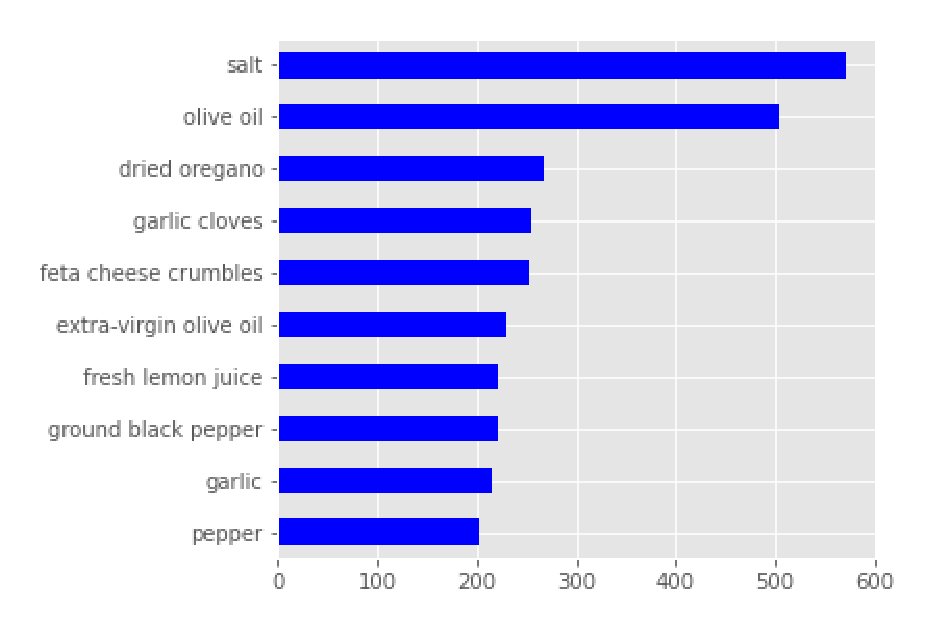
\includegraphics[width=0.5\textwidth]{pic01/greek.eps}
  \end{minipage}
  \begin{minipage}{0.5\linewidth}
    \centering
      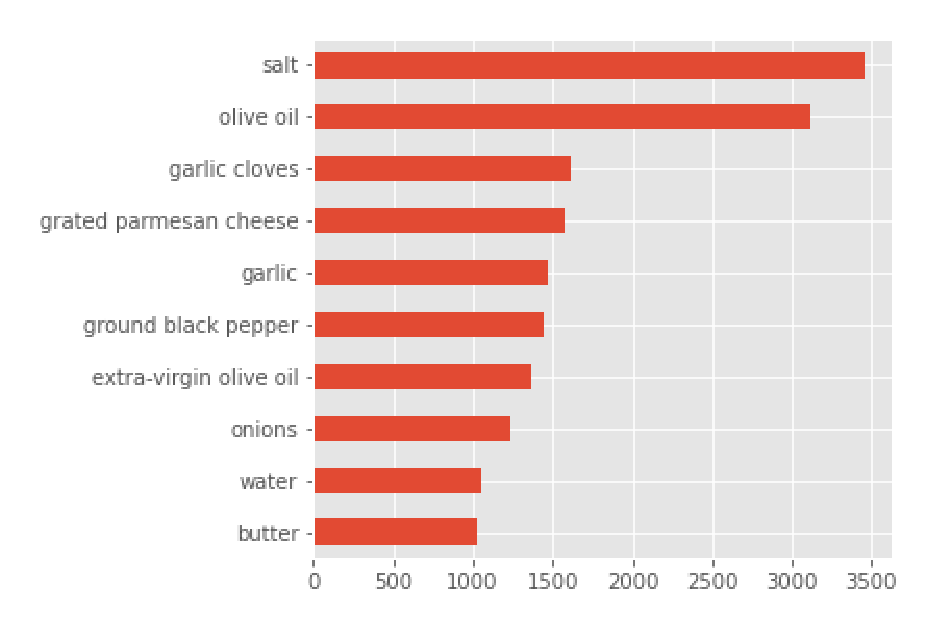
\includegraphics[width=0.5\textwidth]{pic01/italian.eps}
  \end{minipage}
  \hfill
\end{center}


\section{Build Model}
(1)  Data Cleaning:Since dishes contain a large number of ingredients, and since the same ingredients can vary in numbers, tenses, and so on, we considered sifting through a potatos to remove any such differences.
\begin{center}
  \begin{minipage}{1\linewidth}
    \centering
    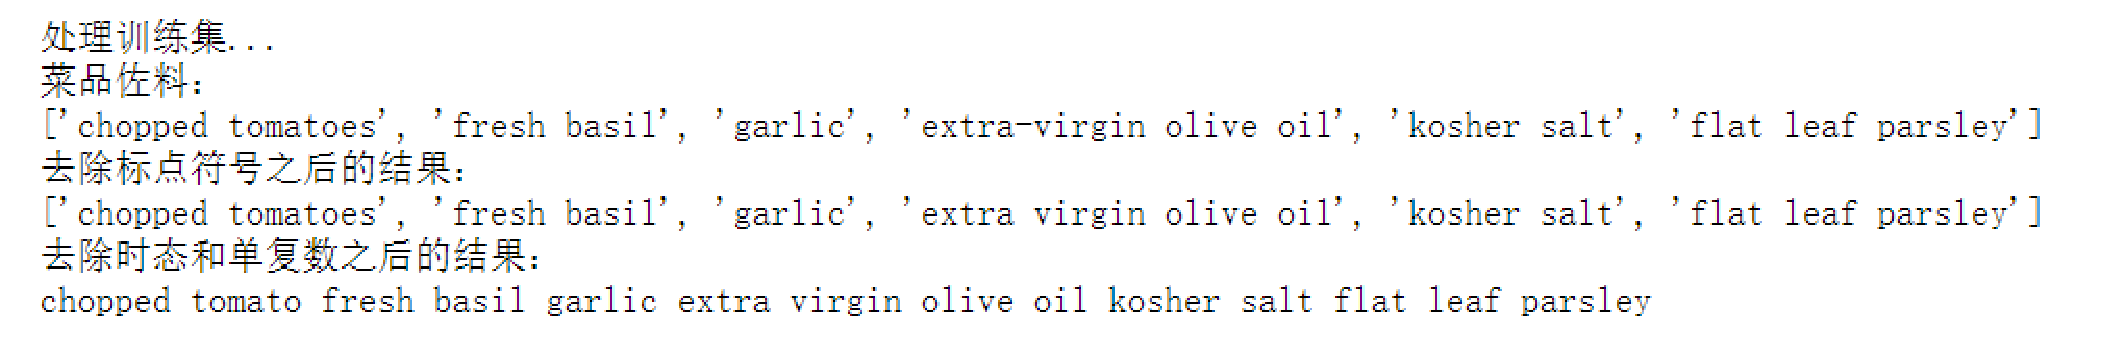
\includegraphics[width=0.9\textwidth]{pic01/clean1.eps}
  \end{minipage}
  \begin{minipage}{1\linewidth}
    \centering
    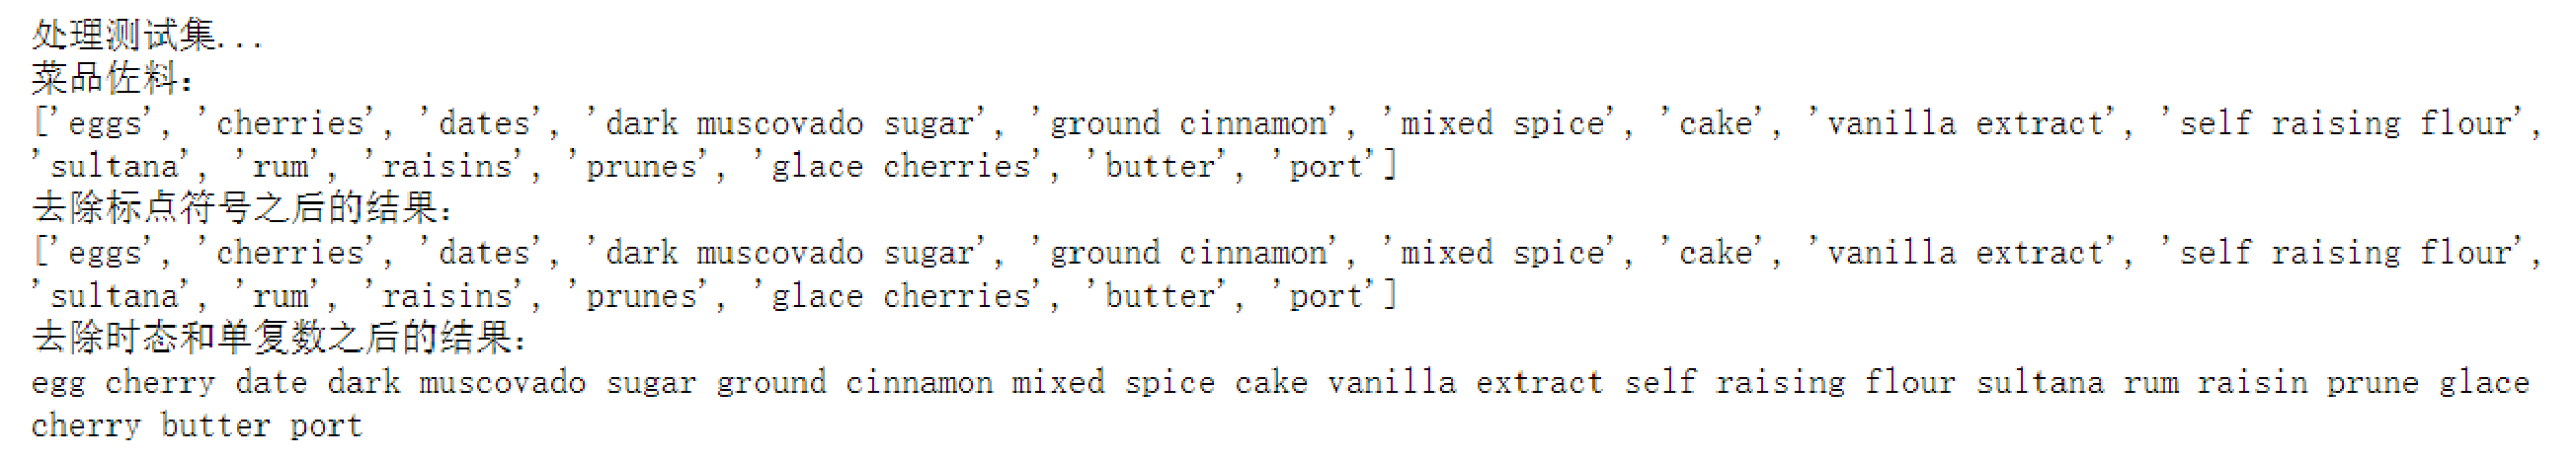
\includegraphics[width=0.9\textwidth]{pic01/clean2.eps}
  \end{minipage}
  
  \hfill
\end{center}
(2) Feature extraction
\begin{itemize}
\item We convert the ingredients of the dish into a numerical feature vector.Consider that most dishes include salt, water, sugar, butter, etc,We will consider weighting the seasonings according to the occurrence times of the seasonings, that is, the more the occurrence times of the condiments, the lower the discriminability of the condiments.The feature we adopt is TF-IDF.
\item We can get the top 5 characteristics:\lbrack'greek','southern\_us','filipino','indian','indian'\rbrack
\item The top five data in train\_tfidf:\\
\lbrack\lbrack0. 0. 0. ... 0. 0. 0.\rbrack\\
\lbrack0. 0. 0. ... 0. 0. 0.\rbrack\\
\lbrack0. 0. 0. ... 0. 0. 0.\rbrack\\
\lbrack0. 0. 0. ... 0. 0. 0.\rbrack\\
\lbrack0. 0. 0. ... 0. 0. 0.\rbrack\rbrack
\end{itemize} 


(3)  Validation set partitioning
\begin{itemize} 
  \item The training set is divided into a new training set and a validation set by calling train_test_split function, which is convenient for the subsequent accuracy observation of the model.
  \item 1.Import train_test_split from sklear.model_selection\\
     2.Use train_tfidf and train_targets as input variables for train_test_split\\
     3.The test_size is set to 0.2, 20$\%$ of the validation set is divided, and 80$\%$ of the data is reserved for the new training set.\\
     4.Set the random_state random seed to ensure that the same partition results are obtained every time you run it.\\
\end{itemize}
(4) Training Model
\begin{itemize} 
       \item Invoke the logistic regression model in sklearn.\\
        1.Import the LogisticRegression from sklear.linear_model.\\
        2.GridSearchCV is imported from sklearn.model_selection, and the parameters are automatically searched. As long as the parameters are typed in, the best results and parameters can be given.\\
        3.Define the parameters variable: Create a dictionary for the C parameters, whose values are an array from 1 to 10;\\
        4.Define the classifier variable: Create a classification function using the imported LogisticRegression;\\
        5.Define Grid variables: Create a grid search object using the imported GridSearchCV;Pass the variables 'classifier', 'parameters' as arguments to the object constructor;
      \item After the model training, we calculated the prediction results of the model on the validation set X_VALID, and calculated the prediction accuracy of the model.
        The score on the validation set is: 0.7958516656191075.\\
\end{itemize}
 
(5)  Predictive test set\\
    Test set test_tfidf is predicted by the model grid, and then the predicted results are viewed.\\
    The predicted number of test sets is 9944.
    \begin{center}
      \begin{minipage}{1\linewidth}
       \centering
       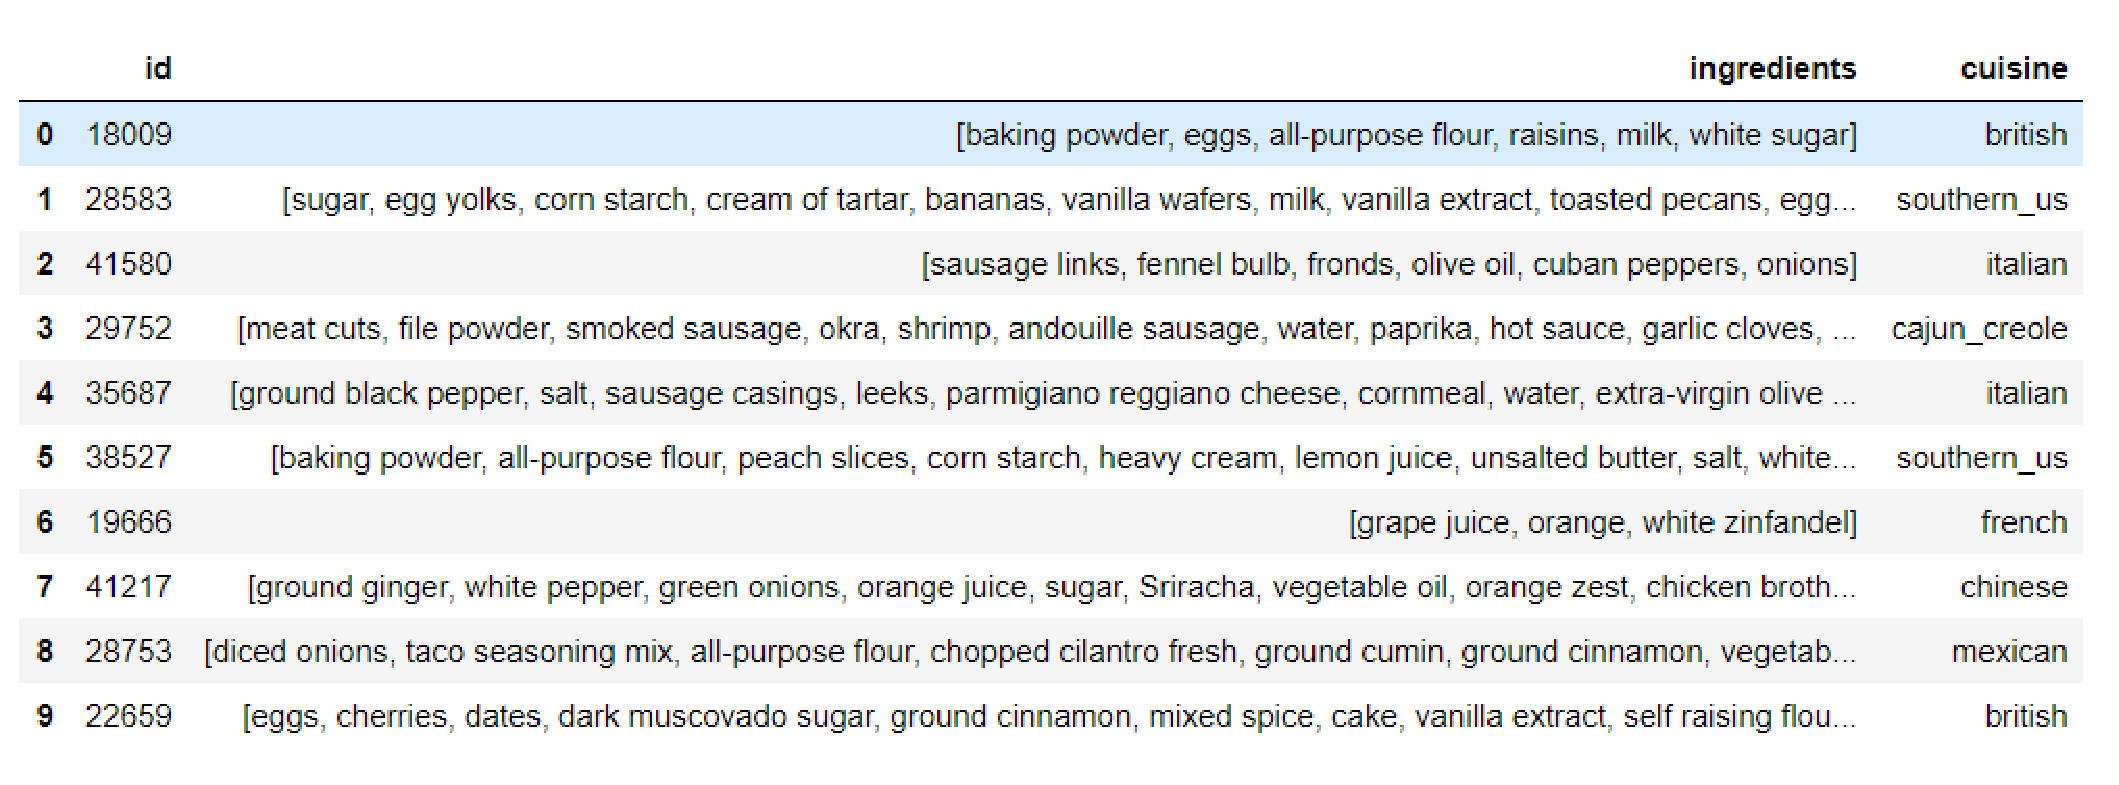
\includegraphics[width=0.7\textwidth]{pic01/result.eps}
      \end{minipage}

      \hfill
    \end{center}

 % \includegraphics[width=0.9\textwidth]{logos/1 (3).eps}
  


